\documentclass{article}[a4]

%\documentclass[preprint]{jasatex}

\usepackage{amsmath,amsfonts}

\usepackage[english]{babel}
\usepackage[caption=false,font=footnotesize]{subfig}
%\usepackage{subfigure}
\usepackage{color}   
\usepackage{booktabs}

\usepackage{graphicx}% Include figure files

% --------------------- end of the preamble ---------------------------

\title{\Large A Method for ultrasound navigation using image data}

\begin{document}

\maketitle

\abstract{This document describes a method for tracking-based fusion
  imaging of real-time ultrasound and computed tomography/magnetic
  resonance (CT/MR images. It is unique in the sense that no absolute
  positioning system is required for the fused CT or MR images to show
  the same plane and move synchronously while performing the real-time
  ultrasound acquisition.}

\section{Background}
Ultrasound is widely used for interventional procedures for the lives
due to a number of advantages; it is non-invasive, easy acessible at a
low cost and most importantly, its real-time capability. Without a
tracking system, the operators need to mentally register previously
acquired CT or MR images to the live ultrasound image. This mental
registration is quite difficult and the situation is further
complicated by the fact that it is often impossible to scan patient
with orthogonal, sagittal or coronal planes, which are used for
interpretation of CT or MR images in the clinic. Due to recent
advances in the CT and MR imaging technologies small target lesions
are often visible only using these modalities and it is of great
interest to fuse the preoperative images with the live ultrasound
images. Using fusion image the operators can conduct interventional
procedures with high confidence and accuracy for challenging target
lesions. Tracking-based image fusion can be realized using an optical or
electromagnetic tracker, where the tracker is responsible for the
absolute positioning after an initial alignment. Fuision imaging has
gained considerable attention and in the BK Medical portfolio of
products we offer a fusion solution for prostate surgery using an
electromagnatic tracker.

\section{Contribution}
The initial alignment of tracker is quite difficult for a number of
reasons. The patient is positioned differently for ultrasound and CT
imaging, e.g. for prostate surgery, the patient is positioned in
Lithotomy, whereas the preoperative CT and MR images are all acquired
while the patient is in Supine position. In general, the different
positioning of the patient results in a deformation and displacement
of organs and it is quite difficult to perform the initial alignment
using image information. This alignment procedure leads directly to
the method that we would like to protect. Real-time tracking of
ultrasound images to preoperative images using image content. The
preoperative images can be MR og CT images but it is not limited to
these modalities. It can even be used for fusing live ultrasound to
previously acquired 3D ultrasound volumes. A situation where this is
useful is for liver tumors requiring overlapping ablations.

\subsection{Alignment}
The alignment of the live ultrasound image to the preoperative content
can be made using algorithms operating directly on the image
data. Such algorithms are very accurate and for registration between different
image modalities, mutual information can be used as a criteria for
correct registration. On a modern desktop computer, 2D registration
using image data can be performed with datarates of more than 50
frames per second. Volume registration is much slower and a couple of
seconds is usually required for registering two volumes to each
other. In Fig.~\ref{fig:fig1}, the result of a registration process
between ultrasound and MR is shown for a 2D prostate image. Methods
using image data are very well suited for registering 2D to 2D or 3D
to 3D, but they are not applicable for registering 2D to 3D. 
\begin{figure}[tbp]
  \centering
  \hfill
  \subfloat[\label{fig:fig1a}]{%
    \resizebox{.31\columnwidth}{!}{%
      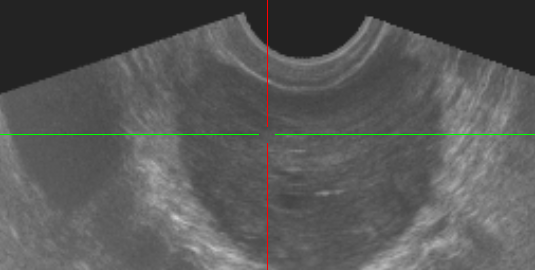
\includegraphics{./us_2D_MI.png}
    }
  }
  \hfill
  \subfloat[\label{fig:fig1b}]{%
    \resizebox{.31\columnwidth}{!}{%
      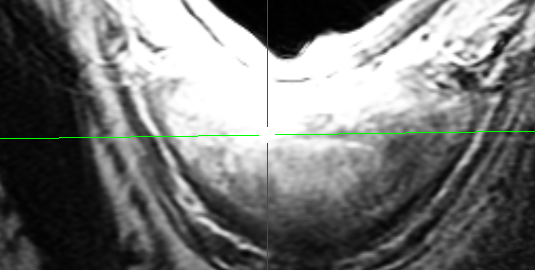
\includegraphics{./mr_2D_MI.png}
    }
  }
  \hfill
  \subfloat[\label{fig:fig1c}]{%
    \resizebox{.31\columnwidth}{!}{%
      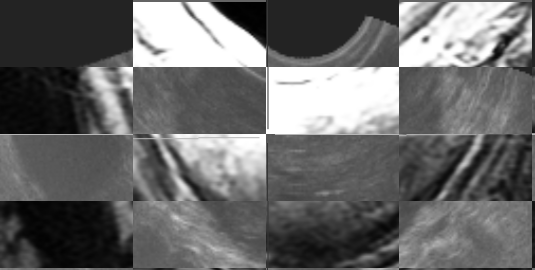
\includegraphics{./MI.png}
    }
  }
  \hfill
  \caption{\protect\subref{fig:fig1a} Ultrasound prostate
    image. \protect\subref{fig:fig1b} MR prostate
    image. \protect\subref{fig:fig1c} Checker pattern demonstrating
    correct registration.}
  \label{fig:fig1}
\end{figure}

Another option is to apply some segmentation for automatically
extracting features present in both the live ultrasound images and the
volume data and perform a registration of the features instead of the
image data. The registration is usually less accurate when compared to
methods using image data, but it is much faster and accuracy can be
acquired by performing multiple registrations and some filtering of
the results. Good features for registration must be visible in both
the preoperative 3D volume and the real-time ultrasound image.

For liver surgery, the vascular tree can be used for registration. In
Fig.~\ref{fig:fig2}, a 2D image showing a bifurcation in the liver is
shown together with a 3D visualization of the features before and
after the registration has been performed. The registration is made
using a simple point-cloud registration algorithm [] and on a modern
desktop computer such registrations can be performed with datarates of more than 100
frames per second.
\begin{figure}[tbp]
  \centering
  \hfill
  \subfloat[\label{fig:fig2a}]{%
    \resizebox{.31\columnwidth}{!}{%
      \includegraphics{./2DImage.png}
    }
  }
  \hfill
  \subfloat[\label{fig:fig2b}]{%
    \resizebox{.31\columnwidth}{!}{%
      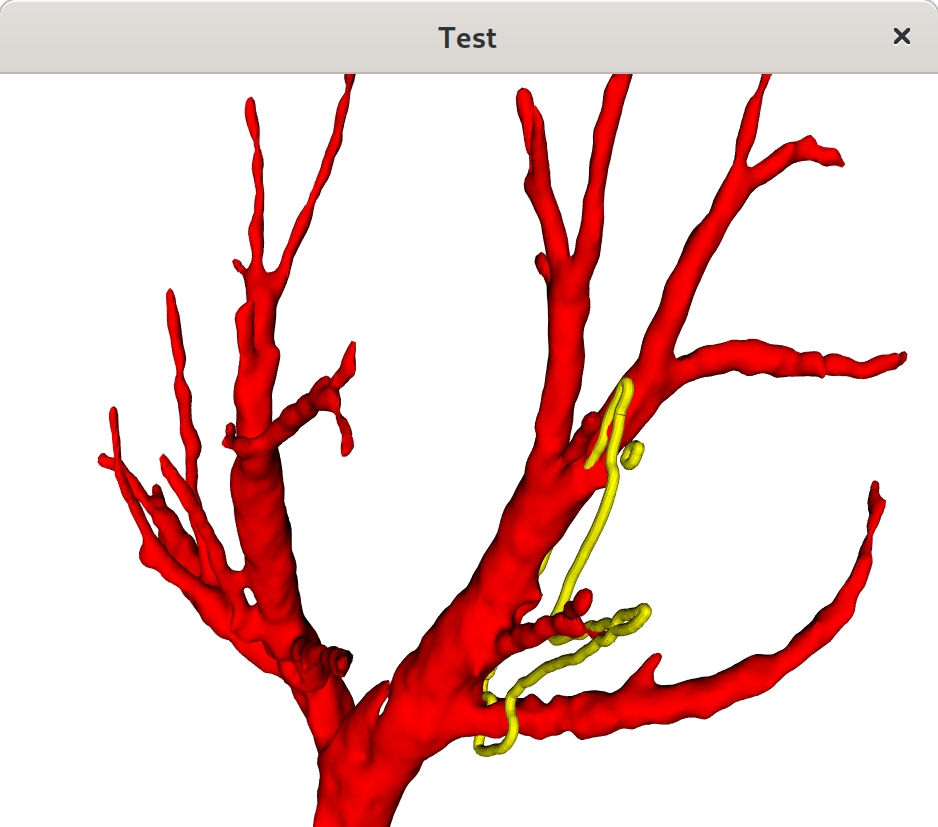
\includegraphics{./VesselOff.png}
    }
  }
  \hfill
  \subfloat[\label{fig:fig2c}]{%
    \resizebox{.31\columnwidth}{!}{%
      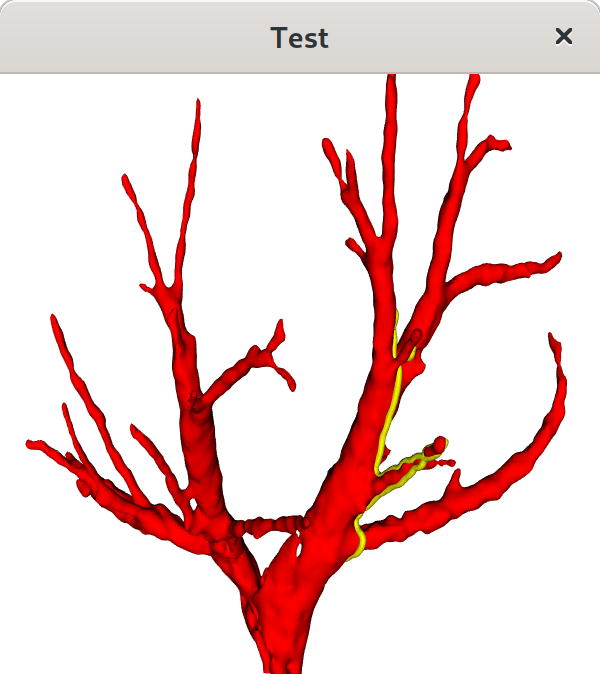
\includegraphics{./VesselPerfect.png}
    }
  }
  \hfill
  \caption{\protect\subref{fig:fig2a} 2D image used for detecting
    contours of vessels. \protect\subref{fig:fig2b} Features
    visualized in 3D for the vascular tree and the contour before
    registration is performed. \protect\subref{fig:fig2c} Features
    visualized after registration.}
  \label{fig:fig2}
\end{figure}

\end{document}
